\chapter{Аналитическая часть}

В данном разделе рассмотрены теоретические выкладки по конвейерной обработке данных и этапам обработки текста: приведению к начальной форме, дедупликации и вычисления частоты терма.

\section{Конвейерная обработка данных}

Конвейер~---~способ обработки данных поэтапно: под каждый этап выделен свой обработчик~---~лента конвейера. Обрабатываемые обработчиком элементы~---~заявки, помещаются в очередь на обработку. После того, как заявка обрабатывается, она помещается в очередь к следующему обработчику.

Пример схемы конвейера представлен на рис.~\ref{img:pipeline_schema}

\begin{figure}[h!]
\centering
    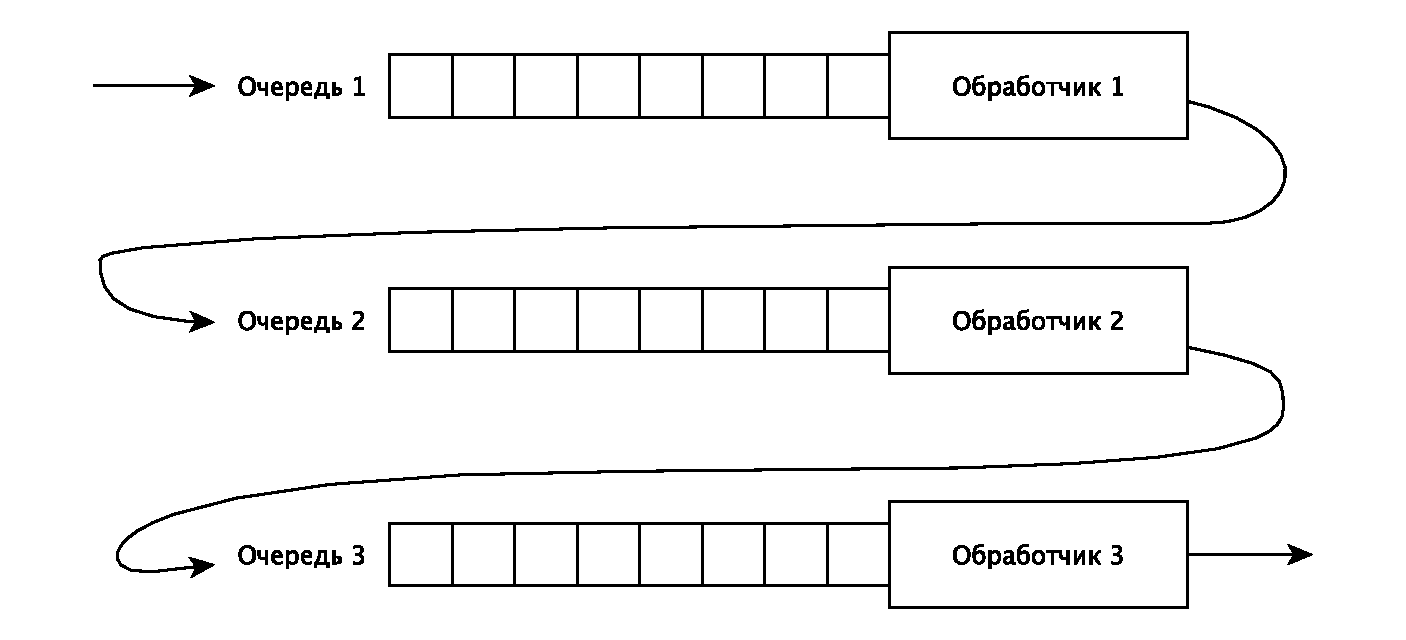
\includegraphics[width=0.8\linewidth]{pipeline_schema.pdf}
    \caption{Схема конвейера}
    \label{img:pipeline_schema}	
\end{figure}

\subsection{Последовательный конвейер}
В последовательном конвейере одновременно может находиться не более одной заявки, то есть пока последний обработчик не вернет заявку, первый не может принять следующую.

\subsection{Параллельный конвейер}
В параллельном конвейере обработчики работают параллельно, или квазипараллельно. Такая схема позволяет находиться и обрабатываться в системе более чем одной заявке.

\section{Этапы обработки текста}

\subsection{Приведение к начальной форме}
Приведение к начальной форме, или нормализация~---~процесс приведения слова к его начальной форме. Пример такого преобразования: <<автомобилем>> $\rightarrow$ <<автомобиль>>.
Приведение к начальной форме необходимо для корректного статистического анализа текста, так как нет смысла рассматривать формы одного и того же слова как отдельные слова. Кроме того, нормализация слов сильно упрощает работу с текстом, в том числе поиск \cite{bib:kazah}. 

\subsection{Дедупликация}
Дедупликация представляет собой удаление дубликатов в наборе. В рамках данной задачи, будет производиться удаление дубликатов в списке терм, то есть слов в начальной форме. Кроме того, будет производится подсчет количества вхождений слова в текст.
 
\subsection{Вычисление частоты терма}
Частота терма $TF$~---~величина, являющаяся характеристикой важности терма в тексте \cite{bib:tf}, которая вычисляется по формуле:

\begin{equation}
	TF = \frac{N_w}{N},
\end{equation}

где
\begin{itemize}
	\item $N_w$~---~количество вхождений данного слова в текст;
	\item $N$~---~количество слов в тексте.
\end{itemize}

\newpage